% Options for packages loaded elsewhere
\PassOptionsToPackage{unicode}{hyperref}
\PassOptionsToPackage{hyphens}{url}
%
\documentclass[
]{book}
\usepackage{lmodern}
\usepackage{amsmath}
\usepackage{ifxetex,ifluatex}
\ifnum 0\ifxetex 1\fi\ifluatex 1\fi=0 % if pdftex
  \usepackage[T1]{fontenc}
  \usepackage[utf8]{inputenc}
  \usepackage{textcomp} % provide euro and other symbols
  \usepackage{amssymb}
\else % if luatex or xetex
  \usepackage{unicode-math}
  \defaultfontfeatures{Scale=MatchLowercase}
  \defaultfontfeatures[\rmfamily]{Ligatures=TeX,Scale=1}
\fi
% Use upquote if available, for straight quotes in verbatim environments
\IfFileExists{upquote.sty}{\usepackage{upquote}}{}
\IfFileExists{microtype.sty}{% use microtype if available
  \usepackage[]{microtype}
  \UseMicrotypeSet[protrusion]{basicmath} % disable protrusion for tt fonts
}{}
\makeatletter
\@ifundefined{KOMAClassName}{% if non-KOMA class
  \IfFileExists{parskip.sty}{%
    \usepackage{parskip}
  }{% else
    \setlength{\parindent}{0pt}
    \setlength{\parskip}{6pt plus 2pt minus 1pt}}
}{% if KOMA class
  \KOMAoptions{parskip=half}}
\makeatother
\usepackage{xcolor}
\IfFileExists{xurl.sty}{\usepackage{xurl}}{} % add URL line breaks if available
\IfFileExists{bookmark.sty}{\usepackage{bookmark}}{\usepackage{hyperref}}
\hypersetup{
  pdftitle={반복측정 자료},
  pdfauthor={서울시립대학교 통계학과 이용희},
  hidelinks,
  pdfcreator={LaTeX via pandoc}}
\urlstyle{same} % disable monospaced font for URLs
\usepackage{color}
\usepackage{fancyvrb}
\newcommand{\VerbBar}{|}
\newcommand{\VERB}{\Verb[commandchars=\\\{\}]}
\DefineVerbatimEnvironment{Highlighting}{Verbatim}{commandchars=\\\{\}}
% Add ',fontsize=\small' for more characters per line
\usepackage{framed}
\definecolor{shadecolor}{RGB}{248,248,248}
\newenvironment{Shaded}{\begin{snugshade}}{\end{snugshade}}
\newcommand{\AlertTok}[1]{\textcolor[rgb]{0.94,0.16,0.16}{#1}}
\newcommand{\AnnotationTok}[1]{\textcolor[rgb]{0.56,0.35,0.01}{\textbf{\textit{#1}}}}
\newcommand{\AttributeTok}[1]{\textcolor[rgb]{0.77,0.63,0.00}{#1}}
\newcommand{\BaseNTok}[1]{\textcolor[rgb]{0.00,0.00,0.81}{#1}}
\newcommand{\BuiltInTok}[1]{#1}
\newcommand{\CharTok}[1]{\textcolor[rgb]{0.31,0.60,0.02}{#1}}
\newcommand{\CommentTok}[1]{\textcolor[rgb]{0.56,0.35,0.01}{\textit{#1}}}
\newcommand{\CommentVarTok}[1]{\textcolor[rgb]{0.56,0.35,0.01}{\textbf{\textit{#1}}}}
\newcommand{\ConstantTok}[1]{\textcolor[rgb]{0.00,0.00,0.00}{#1}}
\newcommand{\ControlFlowTok}[1]{\textcolor[rgb]{0.13,0.29,0.53}{\textbf{#1}}}
\newcommand{\DataTypeTok}[1]{\textcolor[rgb]{0.13,0.29,0.53}{#1}}
\newcommand{\DecValTok}[1]{\textcolor[rgb]{0.00,0.00,0.81}{#1}}
\newcommand{\DocumentationTok}[1]{\textcolor[rgb]{0.56,0.35,0.01}{\textbf{\textit{#1}}}}
\newcommand{\ErrorTok}[1]{\textcolor[rgb]{0.64,0.00,0.00}{\textbf{#1}}}
\newcommand{\ExtensionTok}[1]{#1}
\newcommand{\FloatTok}[1]{\textcolor[rgb]{0.00,0.00,0.81}{#1}}
\newcommand{\FunctionTok}[1]{\textcolor[rgb]{0.00,0.00,0.00}{#1}}
\newcommand{\ImportTok}[1]{#1}
\newcommand{\InformationTok}[1]{\textcolor[rgb]{0.56,0.35,0.01}{\textbf{\textit{#1}}}}
\newcommand{\KeywordTok}[1]{\textcolor[rgb]{0.13,0.29,0.53}{\textbf{#1}}}
\newcommand{\NormalTok}[1]{#1}
\newcommand{\OperatorTok}[1]{\textcolor[rgb]{0.81,0.36,0.00}{\textbf{#1}}}
\newcommand{\OtherTok}[1]{\textcolor[rgb]{0.56,0.35,0.01}{#1}}
\newcommand{\PreprocessorTok}[1]{\textcolor[rgb]{0.56,0.35,0.01}{\textit{#1}}}
\newcommand{\RegionMarkerTok}[1]{#1}
\newcommand{\SpecialCharTok}[1]{\textcolor[rgb]{0.00,0.00,0.00}{#1}}
\newcommand{\SpecialStringTok}[1]{\textcolor[rgb]{0.31,0.60,0.02}{#1}}
\newcommand{\StringTok}[1]{\textcolor[rgb]{0.31,0.60,0.02}{#1}}
\newcommand{\VariableTok}[1]{\textcolor[rgb]{0.00,0.00,0.00}{#1}}
\newcommand{\VerbatimStringTok}[1]{\textcolor[rgb]{0.31,0.60,0.02}{#1}}
\newcommand{\WarningTok}[1]{\textcolor[rgb]{0.56,0.35,0.01}{\textbf{\textit{#1}}}}
\usepackage{longtable,booktabs}
\usepackage{calc} % for calculating minipage widths
% Correct order of tables after \paragraph or \subparagraph
\usepackage{etoolbox}
\makeatletter
\patchcmd\longtable{\par}{\if@noskipsec\mbox{}\fi\par}{}{}
\makeatother
% Allow footnotes in longtable head/foot
\IfFileExists{footnotehyper.sty}{\usepackage{footnotehyper}}{\usepackage{footnote}}
\makesavenoteenv{longtable}
\usepackage{graphicx}
\makeatletter
\def\maxwidth{\ifdim\Gin@nat@width>\linewidth\linewidth\else\Gin@nat@width\fi}
\def\maxheight{\ifdim\Gin@nat@height>\textheight\textheight\else\Gin@nat@height\fi}
\makeatother
% Scale images if necessary, so that they will not overflow the page
% margins by default, and it is still possible to overwrite the defaults
% using explicit options in \includegraphics[width, height, ...]{}
\setkeys{Gin}{width=\maxwidth,height=\maxheight,keepaspectratio}
% Set default figure placement to htbp
\makeatletter
\def\fps@figure{htbp}
\makeatother
\setlength{\emergencystretch}{3em} % prevent overfull lines
\providecommand{\tightlist}{%
  \setlength{\itemsep}{0pt}\setlength{\parskip}{0pt}}
\setcounter{secnumdepth}{5}
%----- my options----------------
\usepackage[hangul]{kotex}
\usepackage{bm}
\usepackage{fullpage}

\newcommand{\pardiff}[2]{\frac{\partial #1}{\partial #2 }}
\newcommand{\pardiffl}[2]{{\partial #1}/{\partial #2 }}
\newcommand{\pardiffd}[2]{\frac{\partial^2 #1}{\partial #2^t \partial #2 }}
\newcommand{\pardiffdd}[3]{\frac{\partial^2 #1}{\partial #2 \partial #3 }}
\newcommand{\norm}[1]{\left\lVert#1\right\rVert}


%--------- from bookdown.org --------------

\usepackage{booktabs}


\usepackage{framed,color}
\definecolor{shadecolor}{RGB}{248,248,248}

\renewcommand{\textfraction}{0.05}
\renewcommand{\topfraction}{0.8}
\renewcommand{\bottomfraction}{0.8}
\renewcommand{\floatpagefraction}{0.75}

\renewenvironment{quote}{\begin{VF}}{\end{VF}}
\let\oldhref\href
\renewcommand{\href}[2]{#2\footnote{\url{#1}}}

\makeatletter
\newenvironment{kframe}{%
\medskip{}
\setlength{\fboxsep}{.8em}
 \def\at@end@of@kframe{}%
 \ifinner\ifhmode%
  \def\at@end@of@kframe{\end{minipage}}%
  \begin{minipage}{\columnwidth}%
 \fi\fi%
 \def\FrameCommand##1{\hskip\@totalleftmargin \hskip-\fboxsep
 \colorbox{shadecolor}{##1}\hskip-\fboxsep
     % There is no \\@totalrightmargin, so:
     \hskip-\linewidth \hskip-\@totalleftmargin \hskip\columnwidth}%
 \MakeFramed {\advance\hsize-\width
   \@totalleftmargin\z@ \linewidth\hsize
   \@setminipage}}%
 {\par\unskip\endMakeFramed%
 \at@end@of@kframe}
\makeatother

\makeatletter

\@ifundefined{Shaded}{
}{\renewenvironment{Shaded}{\begin{kframe}}{\end{kframe}}}
\makeatother

\newenvironment{rmdblock}[1]
  {
  \begin{itemize}
  \renewcommand{\labelitemi}{
    \raisebox{-.7\height}[0pt][0pt]{
      {\setkeys{Gin}{width=3em,keepaspectratio}\includegraphics{images/#1}}
    }
  }
  \setlength{\fboxsep}{1em}
  \begin{kframe}
  \item
  }
  {
  \end{kframe}
  \end{itemize}
  }
  
\newenvironment{rmdnote}
  {\begin{rmdblock}{note}}
  {\end{rmdblock}}
  
\newenvironment{rmdcaution}
  {\begin{rmdblock}{caution}}
  {\end{rmdblock}}
  
\newenvironment{rmdimportant}
  {\begin{rmdblock}{important}}
  {\end{rmdblock}}
  
\newenvironment{rmdtip}
  {\begin{rmdblock}{tip}}
  {\end{rmdblock}}
  
\newenvironment{rmdwarning}
  {\begin{rmdblock}{warning}}
  {\end{rmdblock}}
  


\usepackage{makeidx}
\makeindex

\urlstyle{tt}

\usepackage{amsthm}
\makeatletter
 \def\thm@space@setup{%
   \thm@preskip=8pt plus 2pt minus 4pt
   \thm@postskip=\thm@preskip
}
\makeatother

\frontmatter
\usepackage{booktabs}
\usepackage{longtable}
\usepackage{array}
\usepackage{multirow}
\usepackage{wrapfig}
\usepackage{float}
\usepackage{colortbl}
\usepackage{pdflscape}
\usepackage{tabu}
\usepackage{threeparttable}
\usepackage{threeparttablex}
\usepackage[normalem]{ulem}
\usepackage{makecell}
\usepackage{xcolor}
\ifluatex
  \usepackage{selnolig}  % disable illegal ligatures
\fi
\usepackage[]{natbib}
\bibliographystyle{apalike}

\title{반복측정 자료}
\author{서울시립대학교 통계학과 이용희}
\date{2021-04-16}

\usepackage{amsthm}
\newtheorem{theorem}{Theorem}[chapter]
\newtheorem{lemma}{Lemma}[chapter]
\newtheorem{corollary}{Corollary}[chapter]
\newtheorem{proposition}{Proposition}[chapter]
\newtheorem{conjecture}{Conjecture}[chapter]
\theoremstyle{definition}
\newtheorem{definition}{정의}[chapter]
\theoremstyle{definition}
\newtheorem{example}{예제}[chapter]
\theoremstyle{definition}
\newtheorem{exercise}{Exercise}[chapter]
\theoremstyle{remark}
\newtheorem*{remark}{참고}
\newtheorem*{solution}{Solution}
\begin{document}
\maketitle

{
\setcounter{tocdepth}{1}
\tableofcontents
}
\hypertarget{preface}{%
\chapter*{Preface}\label{preface}}


이 책은 통게학과 대학원생들을 위한 교재이며 고급 의학통계학에 대한 이론과 응용에 대하여 다루고자 합니다.

\begin{rmdimportant}
이 책에서 사용된 기호, 표기법, 프로그램의 규칙과 쓰임은 다음과 같습니다.

\begin{itemize}
\tightlist
\item
  스칼라(scalar)와 일변량 확률변수는 일반적으로 보통 글씨체의 소문자로 표기한다. 특별한 이유가 있는 경우 대문자로 표시할 것이다.
\item
  벡터, 행렬, 다변량 확률벡터는 굵은 글씨체로 표기한다.
\item
  통계 프로그램은 \texttt{SAS}을 이용합니다.
\end{itemize}
\end{rmdimportant}

\mainmatter

\hypertarget{glm}{%
\chapter{반복측정 자료에 대한 모형}\label{glm}}

\hypertarget{uxac1cuxc694}{%
\section{개요}\label{uxac1cuxc694}}

반복측정자료(longitudinal data, repeated measurements)는 관측단위안에서 여러 개의 관측값을 측정한 자료의 형식을 말한다.

예를 들어 환자가 병원을 여러 번 방문하고 방문시마다 혈압을 측정하였다면 한 명의 환자에서 반복 측정한 자료는 서로 독립이 아니다. 또한 가구조사(household survey)에서 가구원의 취업 여부, 건겅 상태등을 여러 해동안 매년 측정하는 경우 이러한 자료를 패널자료(panel data 또는 longitudinal data)라고 한다.

이렇게 하나의 관측단위 안에서 측정한 자료들은 서로 독립이 아닌 특징이 있고 자료를 분석하는 경우 이러한 자료들의 종속구조를 고려하는 모형을 사용하는 것이 적절하다.

이렇게 반복측정자료에서 반복자료들의 공분산구조를 설정하는 통계적 방법들은 다양하지만 대표적으로 쉽게 사용할 수 있는 방법은 전통적인 다변량과 일변량 선형모형을 혼합하여 사용하여 분석할 수 있으며 동시에 임의효과와 오차의 공분산 행렬을 지정할 수 있는 혼합모형을 사용할 수 있다.

\hypertarget{uxbaa8uxd615}{%
\subsection{모형}\label{uxbaa8uxd615}}

\(i\)의 처리를 받은 \(j\) 개체에서 \(k=1,2,\dots,K\)개의 반복 측정을 하였다고 하자. 반응값 \(y_{ijk}\) 에 대한 모형은 다음과 같이 쓸 수 있다.

\begin{equation}
 y_{ijk} = \mu + \alpha_i + \beta_{ij} + \gamma_k + \delta_{ik} + e_{ijk} 
 \label{eq:repeatmodel0}
 \end{equation}

위의 모형에서 각 모수들의 의미는 다음과 같다.

\begin{longtable}[]{@{}cll@{}}
\toprule
\begin{minipage}[b]{(\columnwidth - 2\tabcolsep) * \real{0.36}}\centering
모수\strut
\end{minipage} & \begin{minipage}[b]{(\columnwidth - 2\tabcolsep) * \real{0.32}}\raggedright
의미\strut
\end{minipage} & \begin{minipage}[b]{(\columnwidth - 2\tabcolsep) * \real{0.32}}\raggedright
이름\strut
\end{minipage}\tabularnewline
\midrule
\endhead
\begin{minipage}[t]{(\columnwidth - 2\tabcolsep) * \real{0.36}}\centering
\(\mu\)\strut
\end{minipage} & \begin{minipage}[t]{(\columnwidth - 2\tabcolsep) * \real{0.32}}\raggedright
총 평균\strut
\end{minipage} & \begin{minipage}[t]{(\columnwidth - 2\tabcolsep) * \real{0.32}}\raggedright
grand mean\strut
\end{minipage}\tabularnewline
\begin{minipage}[t]{(\columnwidth - 2\tabcolsep) * \real{0.36}}\centering
\(\alpha_i\)\strut
\end{minipage} & \begin{minipage}[t]{(\columnwidth - 2\tabcolsep) * \real{0.32}}\raggedright
\(i\) 번째 처리 효과\strut
\end{minipage} & \begin{minipage}[t]{(\columnwidth - 2\tabcolsep) * \real{0.32}}\raggedright
treatment effect\strut
\end{minipage}\tabularnewline
\begin{minipage}[t]{(\columnwidth - 2\tabcolsep) * \real{0.36}}\centering
\(\beta_{ij}\)\strut
\end{minipage} & \begin{minipage}[t]{(\columnwidth - 2\tabcolsep) * \real{0.32}}\raggedright
\(i\) 번째 처리 내에서 \(j\)번째 객체의 효과\strut
\end{minipage} & \begin{minipage}[t]{(\columnwidth - 2\tabcolsep) * \real{0.32}}\raggedright
subject effect\strut
\end{minipage}\tabularnewline
\begin{minipage}[t]{(\columnwidth - 2\tabcolsep) * \real{0.36}}\centering
\(\gamma_{k}\)\strut
\end{minipage} & \begin{minipage}[t]{(\columnwidth - 2\tabcolsep) * \real{0.32}}\raggedright
\(k\) 번째 시간의 효과\strut
\end{minipage} & \begin{minipage}[t]{(\columnwidth - 2\tabcolsep) * \real{0.32}}\raggedright
time effect\strut
\end{minipage}\tabularnewline
\begin{minipage}[t]{(\columnwidth - 2\tabcolsep) * \real{0.36}}\centering
\(\delta_{ik}\)\strut
\end{minipage} & \begin{minipage}[t]{(\columnwidth - 2\tabcolsep) * \real{0.32}}\raggedright
\(i\) 번째 처리와 \(k\) 번째 시간의 교효작용 효과\strut
\end{minipage} & \begin{minipage}[t]{(\columnwidth - 2\tabcolsep) * \real{0.32}}\raggedright
interaction between treatment and time\strut
\end{minipage}\tabularnewline
\bottomrule
\end{longtable}

\hypertarget{uxac00uxc124-uxac80uxc815}{%
\subsection{가설 검정}\label{uxac00uxc124-uxac80uxc815}}

다음과 같은 효과에 대한 가설 검정이 반복측정 자료의 분석에서 중요하다.

\begin{itemize}
\item
  between-subject effects (\texttt{trt} )
\item
  within-subject effects (\texttt{time})
\item
  interactions between the two types of effects (\texttt{trt*time})
\end{itemize}

\hypertarget{uxbd84uxd560uxbc95uxc758-uxc751uxc6a9}{%
\section{분할법의 응용}\label{uxbd84uxd560uxbc95uxc758-uxc751uxc6a9}}

반복측정자료는 실험계획법에서 나오는 split-plot 계획을 분석허는 방법을 적용할 수 있다. split-plot 계획의 개념과 분석법은 \href{https://ilovedata.github.io/teaching/experiment/doe-note-w05.pdf}{강의노트}를 참고하시오

다음은 모형식 \eqref{eq:repeatmodel0} 를 분석할 수 있는 일변량 선형모형을 적합하는 \texttt{SAS}의 \texttt{proc\ glm} 프로그램이다.

\begin{verbatim}
proc glm data=bp;
   class trt id time;
   model bp=trt id(trt) time trt*time;
   test h=trt e=id(trt);
run;
\end{verbatim}

위의 프로그램에서 \texttt{id(trt)}은 처리(\texttt{trt}) 안에 개체(\texttt{id})가 내포되어 있다는 모형식이다. 또한 \texttt{test\ h=trt\ e=id(trt)}는 분산분석을 수행할 때 \texttt{trt}에 대한 F-통계량의 분모 오차항을 객체 간의 변동을 나타내는 항으로 사용하라는 명령어이다.

\hypertarget{uxbc18uxbcf5uxce21uxc815-uxbd84uxc0b0uxbd84uxc11d}{%
\section{반복측정 분산분석}\label{uxbc18uxbcf5uxce21uxc815-uxbd84uxc0b0uxbd84uxc11d}}

먼저 \texttt{SAS}의 \texttt{proc\ glm}을 통하여 전통적인 다변량/일변량 선형모형을 사용하여 분석하는 방법을 반복측정 분산분석법(Repeated Measures Analysis of Variance)이라고 한다.

반복측정 분산분석법에 대한 자세한 내용은 \href{https://documentation.sas.com/doc/en/pgmsascdc/9.4_3.3/statug/statug_glm_toc.htm}{SAS 매뉴얼} 와 \href{https://documentation.sas.com/doc/en/pgmsascdc/9.4_3.3/statug/statug_glm_details46.htm}{\texttt{proc\ glm}을 사용한 반복측정 분석}를 참조하자.

\hypertarget{sas-uxc758-proc-glm}{%
\subsection{\texorpdfstring{\texttt{SAS} 의 \texttt{proc\ glm}}{SAS 의 proc glm}}\label{sas-uxc758-proc-glm}}

\texttt{SAS} 의 \texttt{proc\ glm} 은 다변량/일변량 선형모형으로 추론하는 절차를 제공해 준다.

교과서 예제 6.1 에 나오는 자료를 \texttt{SAS} 의 \texttt{proc\ glm}으로 분석하면 다음과 같은 프로그램을 실행한다.

\begin{verbatim}
PROC GLM data=blood_pressure;
   CLASS trt;
   MODEL week0 week4 week8=trt/NOUNI SS3;
   REPEATED week 3(0 4 8 ) CONTRAST(3)/SUMMARY PRINTE ;
 RUN;
\end{verbatim}

위의 \texttt{SAS}프로그램은 다변량을 쉽게 나타낼 수 있는 넓은 형식(wide format)의 자료를 이용한다. 따라서 \texttt{Model} 문장의 식에서 왼쪽 부분은 2개 이상의 변수가 나오며 이 변수들이 반복 측정한 변수들이다.

\texttt{repeated} 는 시간에 대한 변수를 지정하며 반복의 측정 걔수와 간격을 \texttt{3(0\ 4\ 8)}과 같이 지정해준다.

주의할 점은 within-subject effects and interactions 대한 가설 검정은
특별한 가정이 성립해야지 유효하다. 이 가정은 반복측정값들의 공분산이 가지는 구형성 형태(Sphericity)라고 부르며 형태를 가진 공분산은 Type H covariances 라고 부른다.

\begin{verbatim}
  Sphericity is an important assumption of a repeated-measures ANOVA. It is the condition where the variances of the differences between all possible pairs of within-subject conditions (wikidepia)
\end{verbatim}

이러한 가정은 sphericity test (Anderson 1958) 로 검정할 수 있다. Type H covariances 가정이 만족하면 within-subject effects and interactions 대한 가설 검정은 일반적이 F-검정을 사용한다.

만약 만족하지 않는다면 F-검정에서 사용되는 자유도를 수정해 주어야 한다.

sphericity test는 표본의 개수가 작으면 검정력이 떨어지고 표본의 개수가 커지면 너무 많은 제 1 종 오류를 범하는 것으로 알려져 있다. 실제로 자료가 많아지면 구형성을 만족하는 표본 공분산은 거의 없다.

\hypertarget{mixed}{%
\chapter{혼합모형}\label{mixed}}

혼합모형(mixed effect model)은 \texttt{proc\ glm}에서 나타나는 모든 선형모형을 포함한 더욱 다양한 모형을 적합할 수 있다. 모수의 추정 방법은 최소제곱법이 아닌 최대가능도 추정법을 이용한다.

\begin{rmdimportant}
반복측정자료에 최소제곱법을 사용하는 경우 결측값을 가진 개체는 분석에서 제외된다. 반면 혼합모형은 결측값이 있는 개체도 분석에 포함하여 추론이 가능하다.
\end{rmdimportant}

혼합모형에서 일반적인 모형의 정의는 다음과 같다.

\begin{equation}
\bm y = \bm X  \bm \beta + \bm Z \bm b + \bm e 
\label{eq:mixedmodel}
\end{equation}

위의 모형식에 대한 항들의 역할은 다음과 같다.

\begin{longtable}[]{@{}cll@{}}
\toprule
식의 요소 & 의미 & 이름\tabularnewline
\midrule
\endhead
\(\bm y\) & 반응변수 벡터 & response vector\tabularnewline
\(\bm X\) & 고정효과에 대한 계획행렬 & design matrix for fixed effects\tabularnewline
\(\bm \beta\) & 고정효과 벡터(모수) & fixed effect(parameters)\tabularnewline
\(\bm Z\) & 임의효과에 대한 계획행렬 & design matrix for random effect\tabularnewline
\(\bm b\) & 임의효과 벡터 & random effect\tabularnewline
\(\bm e\) & 오차 벡터 & error vector\tabularnewline
\bottomrule
\end{longtable}

혼합모형에서 임의효과 \(\bm b\) 와 오차항 \(\bm e\) 에 대한 분포 가정은 다음과 같다.

\begin{equation}
\bm b \sim N( \bm 0, \bm G), \quad \bm e \sim N(\bm 0, \bm R)
\label{eq:mixedassume}
\end{equation}

또한 임의효과 \(\bm b\) 와 오차항 \(\bm e\) 은 서로 독립니다.

\[ Cov( \bm b, \bm e) = \bm 0 \]

모형이 식 \eqref{eq:mixedmodel} 인 경우 경우 관측벡터의 공분산의 다음과 같이 주어진다.

\[ Var( \bm y) = \bm Z^t \bm G \bm Z + \bm R \]

임의 효과 벡터 \(\bm b\)는 일반적으로 개체들이 깉은 그룹에 속하는 계층적인
효과를 반영하기 위하여 사용된다. 쯕, 같은 그룹이나 클러스터에 속하는 개체는 공통의 임의 효과를 공유하게 되어 서로 독립이 아니게 된다. 따라서 임의 효과 벡터 \(\bm b\)의 공분산 행렬 \(\bm G\)에서 개체들의 종속적인 구조를 나타낸다.

오차항에 대한 공분산 행렬 \(\bm R\)은 하나의 개체에서 관측되는 여러개의 관측값들이 독립이 아닌 경우 어떻게 연관되는 지를 나타낸다. 보통 오차들이 시간과 공간에 따라 나타날 수 있는 상관관계를 구조화하는 행렬이다.

오차항에 대한 공분산 행렬 \(\bm R\)은 \(\sigma^2 \bm I\)로 가정한는 경우가 많다. 일반적으로 오차항은 모두 독립이며 개체들의 종속성은 그 개체들이 속하는 그룹의 계층적인 구조에서 나온다고 가정한다. 특별하게 반복측정에서 오는 시계열적인 구조나 공간구조에 따르는 종속성이 나타나는 문제에서는 공분산 행렬 \(\bm R\)을 특수한 행렬로 보고 추정할 수 있다.

\hypertarget{uxc608uxc81c-uxc784uxc758-uxacc4uxc218-uxbaa8uxd615}{%
\section{예제: 임의 계수 모형}\label{uxc608uxc81c-uxc784uxc758-uxacc4uxc218-uxbaa8uxd615}}

\begin{example}[Sleep study]
\protect\hypertarget{exm:unnamed-chunk-5}{}{\label{exm:unnamed-chunk-5} \iffalse (Sleep study) \fi{} }\texttt{lme4} 패키지에 자료인 \texttt{spleepstudy}는 화물트럭 운전사들에 대한 수면부족 현상에 대하여 연구한 자료이다. 18명의 운전자들이 매일 3시간의 수면(부족한 수면)을 하면서
매일 일정한 동작의 반응시간을 10일동안 반복적으로 측정한 자료가 있다. 한명의 운전사에게 10일 동안의 반응에 대한 측정자료 10개가 존재하므로 이는 반복측정 자료이며 이러한 10개의 자료는 독립이 아니다.
일단 자료의 구조를 살펴보자. 반응변수 \texttt{Reaction}은 반응시간(ms)를 나타내며 설명변수로서 \texttt{Days}는 날짜(\(t=0,1,2,\dots,9\)), \texttt{Subject}는 운전자의 고유번호를 나타낸다.
\end{example}

\begin{center}\rule{0.5\linewidth}{0.5pt}\end{center}

\begin{Shaded}
\begin{Highlighting}[]
\FunctionTok{library}\NormalTok{(lme4)}
\end{Highlighting}
\end{Shaded}

\begin{verbatim}
## Loading required package: Matrix
\end{verbatim}

\begin{verbatim}
## 
## Attaching package: 'Matrix'
\end{verbatim}

\begin{verbatim}
## The following objects are masked from 'package:tidyr':
## 
##     expand, pack, unpack
\end{verbatim}

\begin{Shaded}
\begin{Highlighting}[]
\FunctionTok{str}\NormalTok{(sleepstudy)}
\end{Highlighting}
\end{Shaded}

\begin{verbatim}
## 'data.frame':    180 obs. of  3 variables:
##  $ Reaction: num  250 259 251 321 357 ...
##  $ Days    : num  0 1 2 3 4 5 6 7 8 9 ...
##  $ Subject : Factor w/ 18 levels "308","309","310",..: 1 1 1 1 1 1 1 1 1 1 ...
\end{verbatim}

\begin{Shaded}
\begin{Highlighting}[]
\FunctionTok{head}\NormalTok{(sleepstudy,}\AttributeTok{n=}\DecValTok{20}\NormalTok{)}
\end{Highlighting}
\end{Shaded}

\begin{verbatim}
##    Reaction Days Subject
## 1  249.5600    0     308
## 2  258.7047    1     308
## 3  250.8006    2     308
## 4  321.4398    3     308
## 5  356.8519    4     308
## 6  414.6901    5     308
## 7  382.2038    6     308
## 8  290.1486    7     308
## 9  430.5853    8     308
## 10 466.3535    9     308
## 11 222.7339    0     309
## 12 205.2658    1     309
## 13 202.9778    2     309
## 14 204.7070    3     309
## 15 207.7161    4     309
## 16 215.9618    5     309
## 17 213.6303    6     309
## 18 217.7272    7     309
## 19 224.2957    8     309
## 20 237.3142    9     309
\end{verbatim}

각 운전자에 대한 10일 간의 반응속도가 시간에 따라 어떻게 변하는 가를 알아보자. 전반적으로 시간이 지나면서 운전자들의 반응시간이 증가하고 있음을 알 수 있다. 또한 개인 별로 반응 시간의 변화와 패턴이 다르다는 것을 알 수 있다.

\begin{Shaded}
\begin{Highlighting}[]
\FunctionTok{library}\NormalTok{(ggplot2)}
\FunctionTok{ggplot}\NormalTok{(sleepstudy, }\FunctionTok{aes}\NormalTok{(}\AttributeTok{x=}\NormalTok{Days, }\AttributeTok{y=}\NormalTok{Reaction)) }\SpecialCharTok{+}
     \FunctionTok{geom\_point}\NormalTok{(}\AttributeTok{size=}\FloatTok{0.5}\NormalTok{) }\SpecialCharTok{+}
     \FunctionTok{stat\_smooth}\NormalTok{(}\AttributeTok{method =} \StringTok{"lm"}\NormalTok{,}\AttributeTok{se=}\NormalTok{F,}\AttributeTok{size=}\FloatTok{0.5}\NormalTok{)}\SpecialCharTok{+}
     \FunctionTok{facet\_wrap}\NormalTok{(}\StringTok{"Subject"}\NormalTok{, }\AttributeTok{labeller =}\NormalTok{ label\_both)}\SpecialCharTok{+} 
     \FunctionTok{theme\_bw}\NormalTok{()}
\end{Highlighting}
\end{Shaded}

\begin{verbatim}
## `geom_smooth()` using formula 'y ~ x'
\end{verbatim}

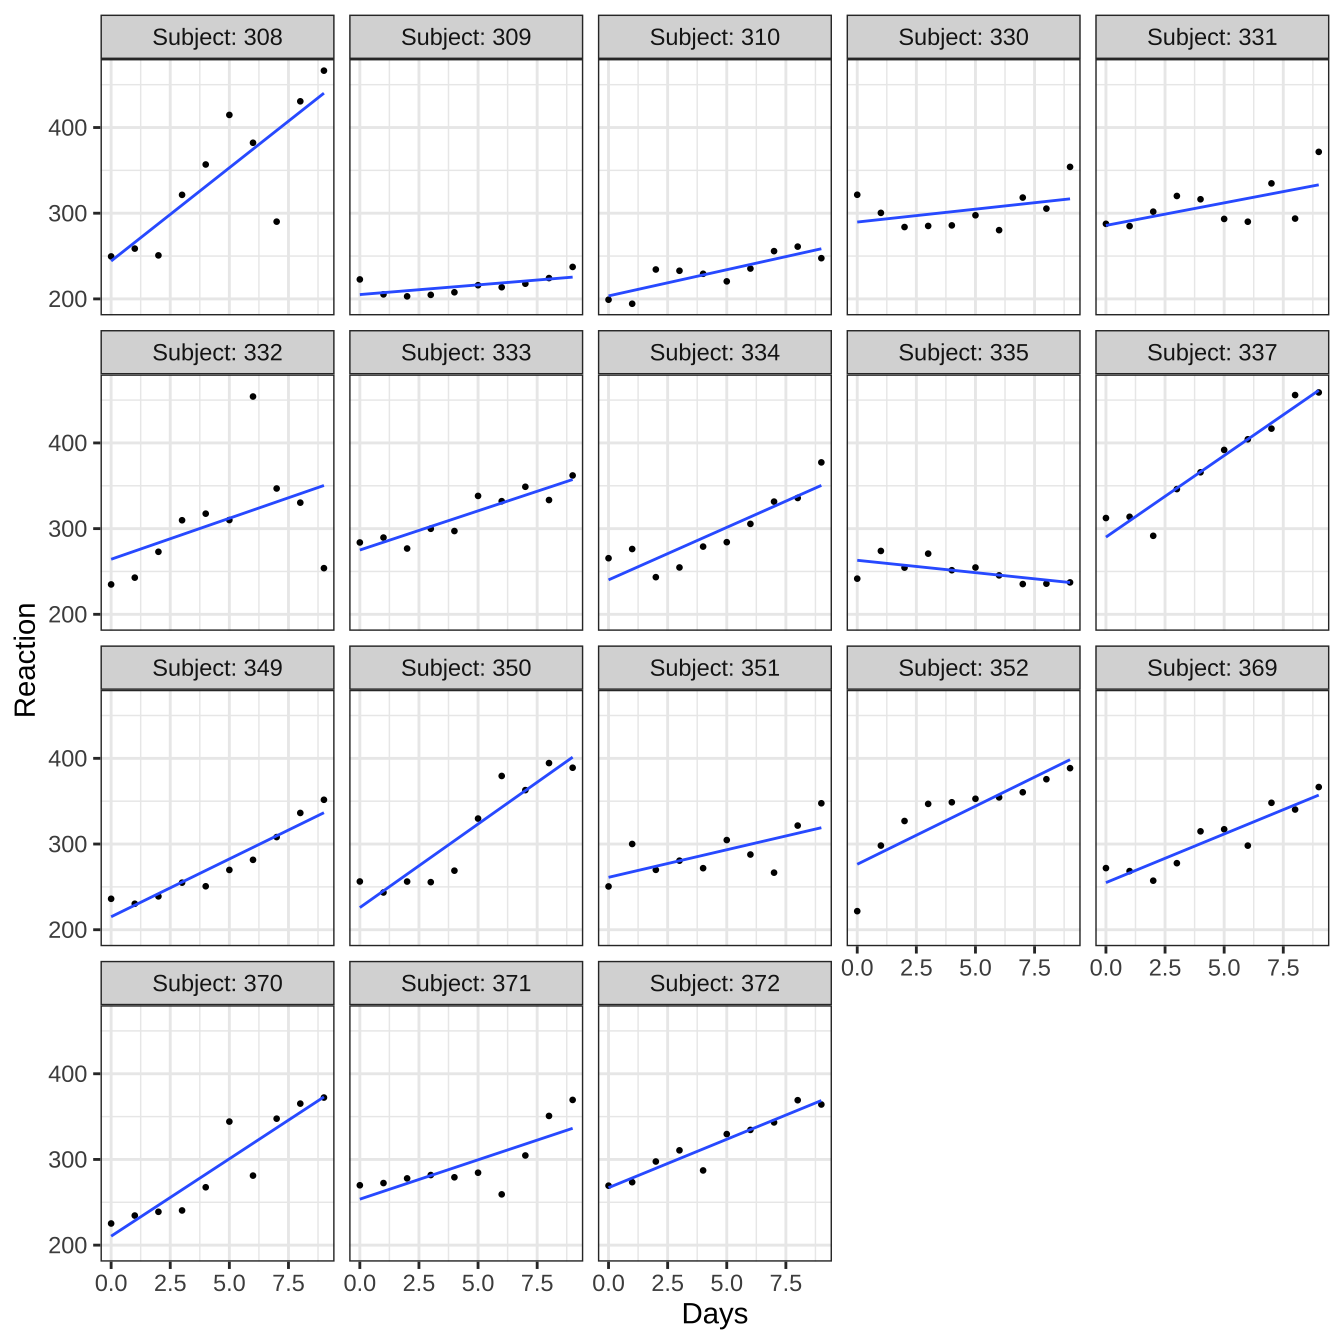
\includegraphics[width=.8\linewidth]{repeat_files/figure-latex/ex15-1}

\hypertarget{uxac1cuxccb4uxb4e4uxc758-uxc120uxd615-uxd68cuxadc0uxbaa8uxd615}{%
\subsection{개체들의 선형 회귀모형}\label{uxac1cuxccb4uxb4e4uxc758-uxc120uxd615-uxd68cuxadc0uxbaa8uxd615}}

각 운전자 \(i\) 에 대하여 10일간 측정한 반응속도 \(y_{ij}\)를 시간에 대하여 선형모형으로 적합하면 개인별 회귀직선을 다음과 같이 표시할 수 있다.

\begin{equation}
y_{ij} = \beta_{0i} + \beta_{1i} t_j + e_{ij},\quad i=1,2,\dots,18,\quad j=1,2,\dots,10
\label{eq:lmlist1}
\end{equation}

여기서 오차항 \(e_{ij}\)은 서로 독립이며 \(N(0, \sigma^2_e)\)를 따른다고 가정한다.

행렬식으로는 다음과 같이 나타낼 수 있다.

\[ 
\bm y_i =\bm X_i \bm \beta_{i} +\bm e_i 
\]

여기서
\[
\bm y_i=\left[ \begin{array}{c}
y_{i1} \\
y_{i2} \\
\vdots \\
y_{i,10}
\end{array} \right],~ \bm X_i =
\left[ \begin{array}{cc}
1 & 0 \\
1 & 1 \\
\vdots & \vdots  \\
1 & 9 
\end{array} \right], \bm \beta_i=
\left[ \begin{array}{c}
\beta_{0i} \\
\beta_{1i} \\
\end{array} \right], \bm e_i= 
\left[ \begin{array}{c}
e_{i1} \\
e_{i2} \\
\vdots \\
e_{i,10}
\end{array} \right]
\]

위의 식에서 \(\beta_{0i}\)와 \(\beta_{1i}\)는 \(i\)번째 운전사의 반응속도를 설명내는 회귀직선의 절편과 기울기이다. 절편 \(\beta_{0i}\)는 실험 시작때 반응속도를 의미하고 기울기 \(\beta_{1i}\)는 실험이 진행되는 동안 반응속도가 어떻게 변하는 지 변화의 방향과 크기를 보여준다. 함수 \texttt{lmList}를 아래와 같이 이용하면 식 \eqref{eq:lmlist1} 을 각 운전사마다 적합시켜 각각의 절편과 기울기를 구할 수 있다.

\begin{Shaded}
\begin{Highlighting}[]
\NormalTok{lmf1 }\OtherTok{\textless{}{-}} \FunctionTok{lmList}\NormalTok{(Reaction }\SpecialCharTok{\textasciitilde{}}\NormalTok{ Days }\SpecialCharTok{|}\NormalTok{ Subject, sleepstudy)}
\NormalTok{lmf1}
\end{Highlighting}
\end{Shaded}

\begin{verbatim}
## Call: lmList(formula = Reaction ~ Days | Subject, data = sleepstudy) 
## Coefficients:
##     (Intercept)      Days
## 308    244.1927 21.764702
## 309    205.0549  2.261785
## 310    203.4842  6.114899
## 330    289.6851  3.008073
## 331    285.7390  5.266019
## 332    264.2516  9.566768
## 333    275.0191  9.142045
## 334    240.1629 12.253141
## 335    263.0347 -2.881034
## 337    290.1041 19.025974
## 349    215.1118 13.493933
## 350    225.8346 19.504017
## 351    261.1470  6.433498
## 352    276.3721 13.566549
## 369    254.9681 11.348109
## 370    210.4491 18.056151
## 371    253.6360  9.188445
## 372    267.0448 11.298073
## 
## Degrees of freedom: 180 total; 144 residual
## Residual standard error: 25.59182
\end{verbatim}

\begin{Shaded}
\begin{Highlighting}[]
\FunctionTok{cor}\NormalTok{(}\FunctionTok{coef}\NormalTok{(lmf1))}
\end{Highlighting}
\end{Shaded}

\begin{verbatim}
##             (Intercept)       Days
## (Intercept)   1.0000000 -0.1375534
## Days         -0.1375534  1.0000000
\end{verbatim}

\begin{Shaded}
\begin{Highlighting}[]
\FunctionTok{plot}\NormalTok{(}\FunctionTok{coef}\NormalTok{(lmf1),}\AttributeTok{main=}\StringTok{"intercepts and slopes on drivers: sleep study "}\NormalTok{)}
\end{Highlighting}
\end{Shaded}

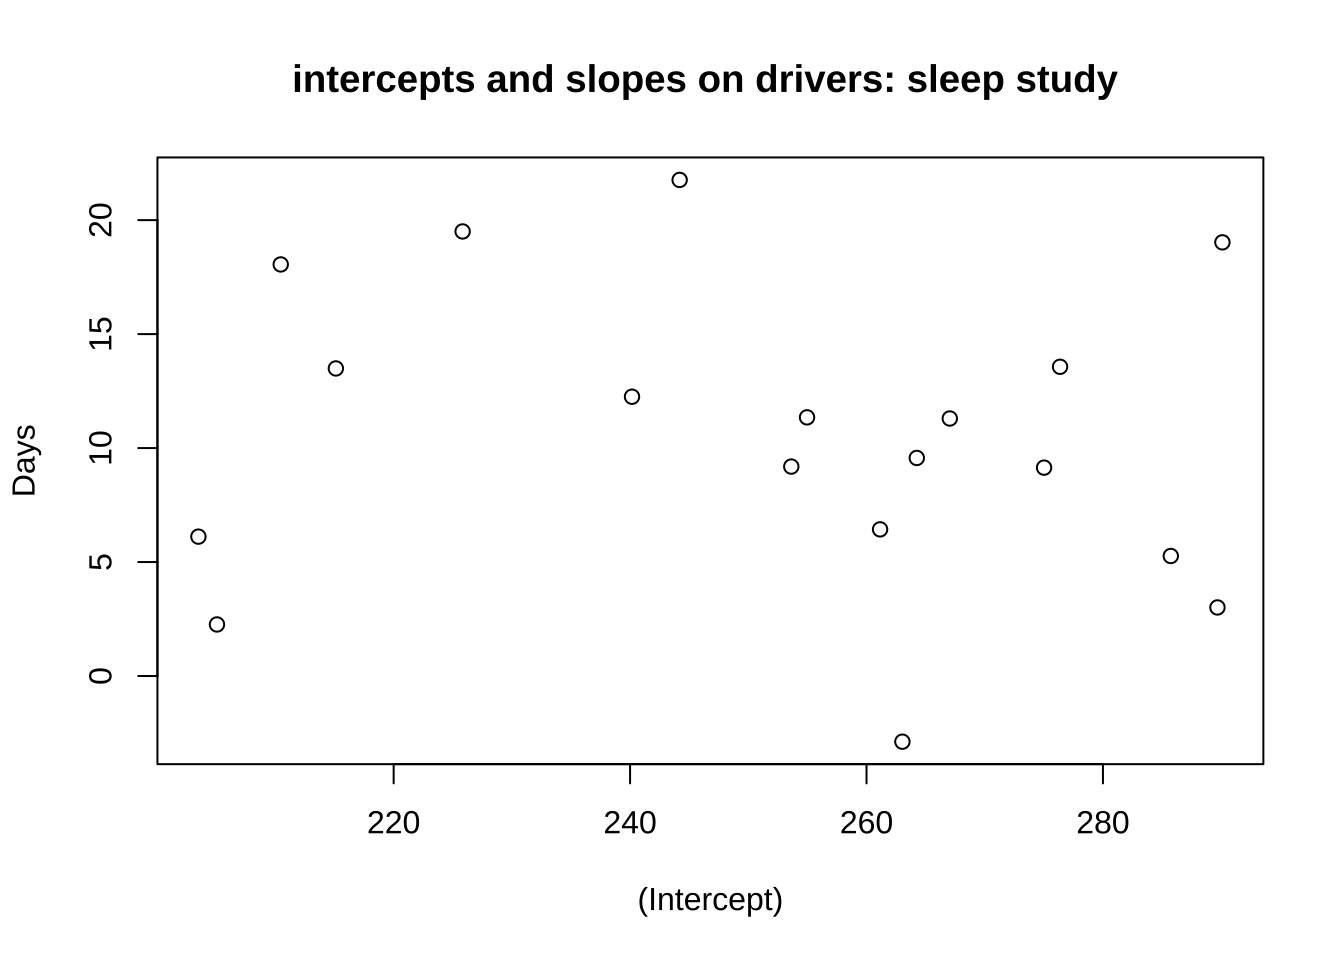
\includegraphics[width=.8\linewidth]{repeat_files/figure-latex/ex16-1}

18개의 절편과 기울기는 큰 상관관계는 없는것으로 보이지만 약한 음의 상관계수가 나타났다.\\
절편과 기울기에 대한 분포를 보기 위하여 상자그림을 그려보면 평균을 중심으로 대칭인 분포를 보이고 있다.

\begin{Shaded}
\begin{Highlighting}[]
\FunctionTok{boxplot}\NormalTok{(}\FunctionTok{coef}\NormalTok{(lmf1)[}\DecValTok{1}\NormalTok{])}
\FunctionTok{boxplot}\NormalTok{(}\FunctionTok{coef}\NormalTok{(lmf1)[}\DecValTok{2}\NormalTok{])}
\end{Highlighting}
\end{Shaded}

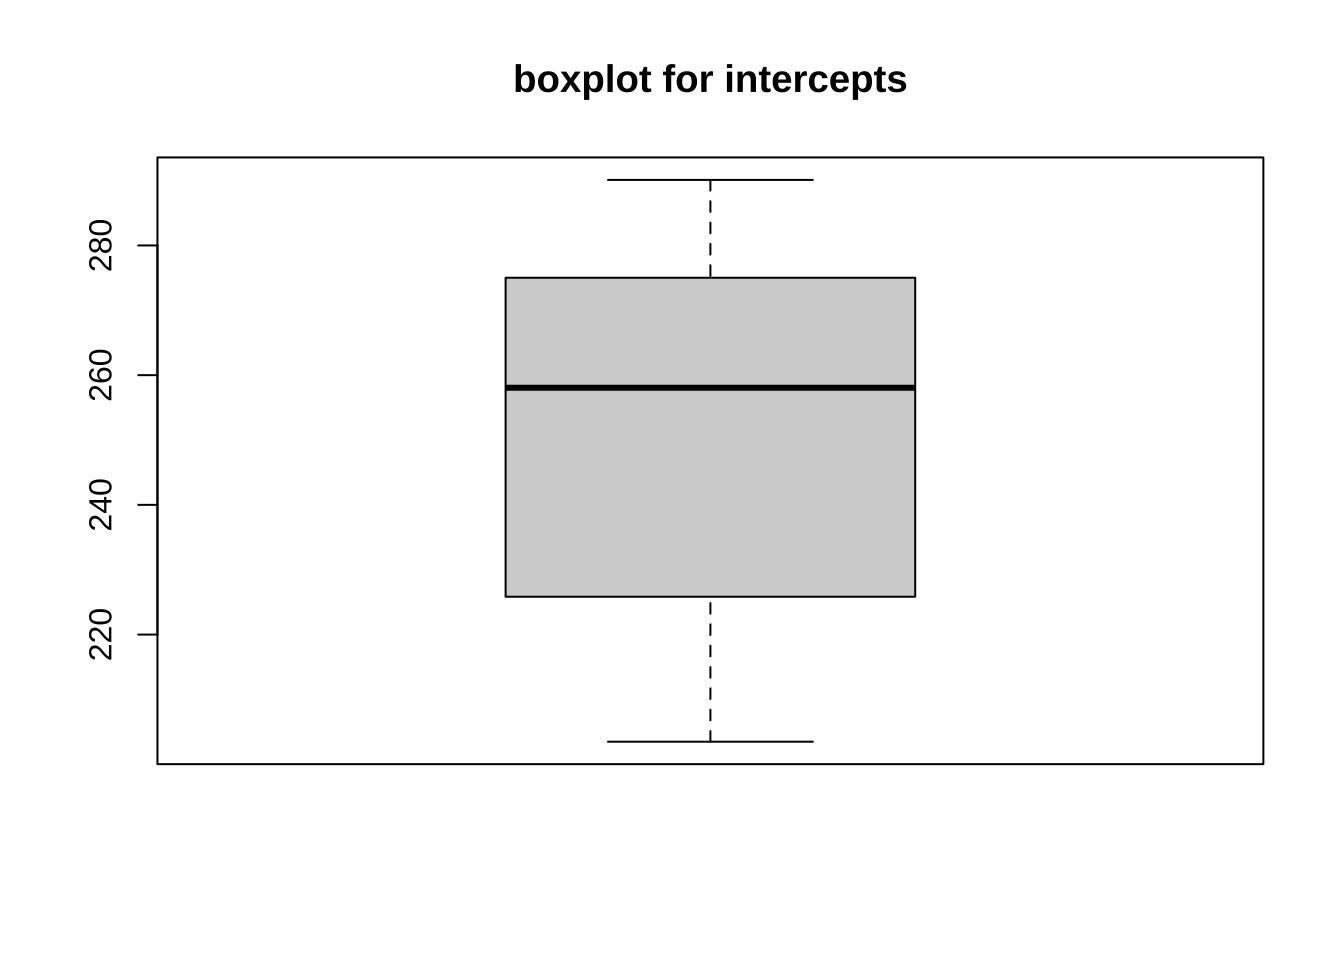
\includegraphics[width=6cm,height=6cm]{repeat_files/figure-latex/box-1} 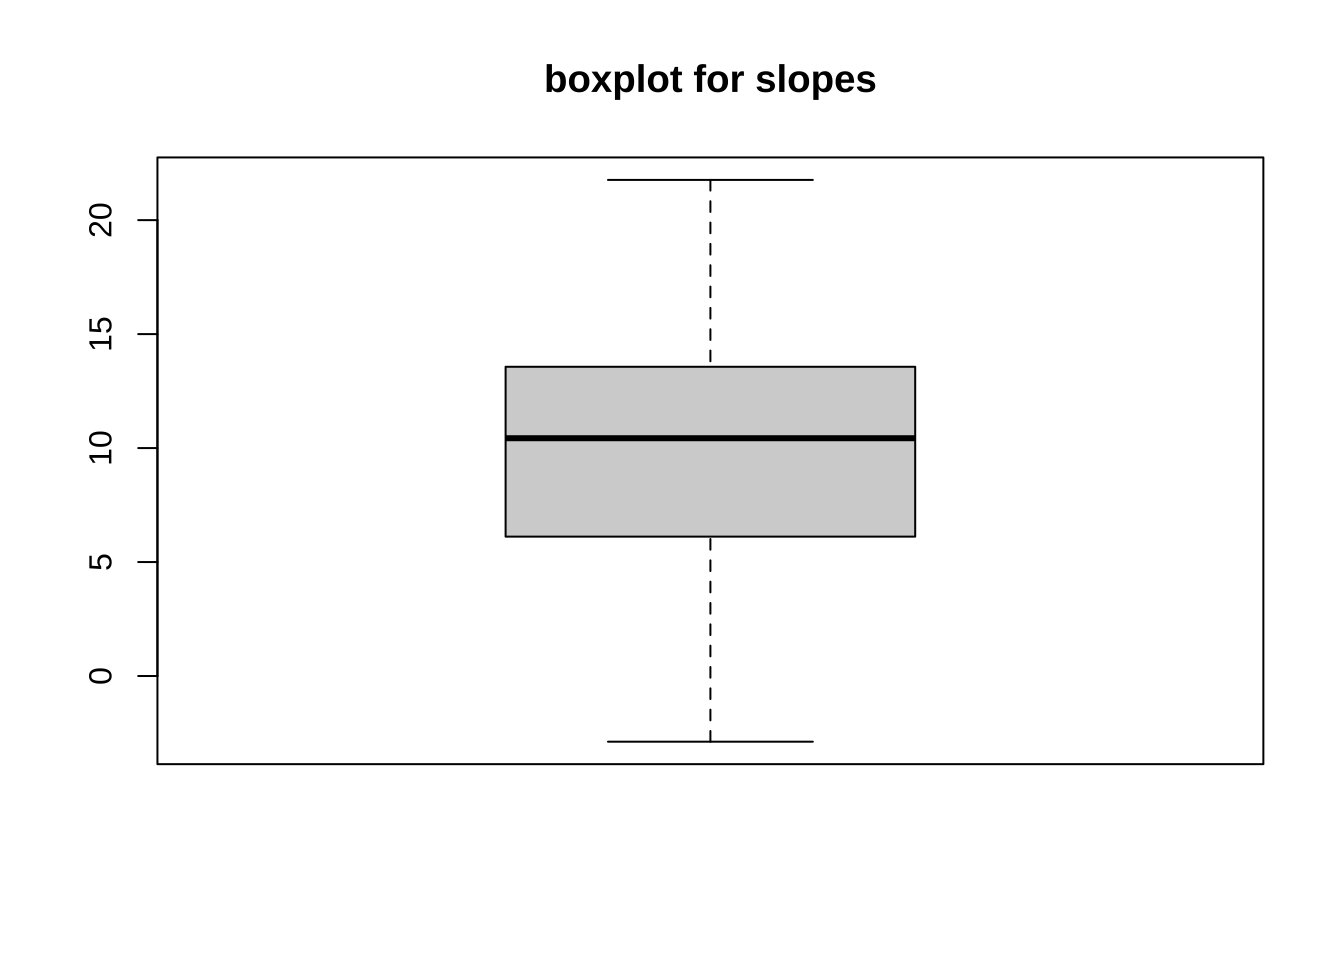
\includegraphics[width=6cm,height=6cm]{repeat_files/figure-latex/box-2}

이제 각 운전사에 대하여 회귀식을 따로 적합하지 않고 전체 운전사들의 자료를 모두 합쳐서 하나의 회귀식을 고려할 수 있다. 개체의 특성을 반영하는 모형이 아닌 전체 집단에 대한 평균적인 모형(population model)을 고려하는 것이다.

\begin{equation} 
y_{ij} = \beta_0 + \beta_1 t_j + e_{ij} ,\quad i=1,2\dots,18,  j=1,2, \dots, 10 
\label{eq:popmodel}
\end{equation}

여기서 오차항은 서로 독립이며 \(N(0, \sigma^2_e)\)를 따른다고 가정한다.

위와 같은 전체 운전사 집단의 관측값을 운전자의 특성을 고려하지 않고 세운 모형으로서 시간에 따른 반응시간에 대한 모집단의 전체적인 평균적 함수 관계를 파악하는 모형이라고 할 수 있다.

\begin{Shaded}
\begin{Highlighting}[]
\NormalTok{lmpop }\OtherTok{\textless{}{-}} \FunctionTok{lm}\NormalTok{(Reaction }\SpecialCharTok{\textasciitilde{}}\NormalTok{ Days, sleepstudy)}
\FunctionTok{summary}\NormalTok{(lmpop)}
\end{Highlighting}
\end{Shaded}

\begin{verbatim}
## 
## Call:
## lm(formula = Reaction ~ Days, data = sleepstudy)
## 
## Residuals:
##      Min       1Q   Median       3Q      Max 
## -110.848  -27.483    1.546   26.142  139.953 
## 
## Coefficients:
##             Estimate Std. Error t value Pr(>|t|)    
## (Intercept)  251.405      6.610  38.033  < 2e-16 ***
## Days          10.467      1.238   8.454 9.89e-15 ***
## ---
## Signif. codes:  0 '***' 0.001 '**' 0.01 '*' 0.05 '.' 0.1 ' ' 1
## 
## Residual standard error: 47.71 on 178 degrees of freedom
## Multiple R-squared:  0.2865, Adjusted R-squared:  0.2825 
## F-statistic: 71.46 on 1 and 178 DF,  p-value: 9.894e-15
\end{verbatim}

\begin{Shaded}
\begin{Highlighting}[]
\FunctionTok{with}\NormalTok{(sleepstudy, }\FunctionTok{plot}\NormalTok{(Days, Reaction,}\AttributeTok{main=}\StringTok{"Population and individual regression lines"}\NormalTok{))}
\FunctionTok{abline}\NormalTok{(}\AttributeTok{a=}\FunctionTok{coef}\NormalTok{(lmpop)[}\DecValTok{1}\NormalTok{], }\AttributeTok{b=}\FunctionTok{coef}\NormalTok{(lmpop)[}\DecValTok{2}\NormalTok{],}\AttributeTok{lwd=}\DecValTok{3}\NormalTok{)}
\ControlFlowTok{for}\NormalTok{ ( i }\ControlFlowTok{in} \DecValTok{1}\SpecialCharTok{:}\DecValTok{18}\NormalTok{ ) \{}
\NormalTok{  xx }\OtherTok{\textless{}{-}} \FunctionTok{as.numeric}\NormalTok{(}\FunctionTok{coef}\NormalTok{(lmf1)[i,])}
\FunctionTok{abline}\NormalTok{(}\AttributeTok{a=}\NormalTok{xx[}\DecValTok{1}\NormalTok{],}\AttributeTok{b=}\NormalTok{xx[}\DecValTok{2}\NormalTok{], }\AttributeTok{lty=}\DecValTok{2}\NormalTok{)}
\NormalTok{\}}
\end{Highlighting}
\end{Shaded}

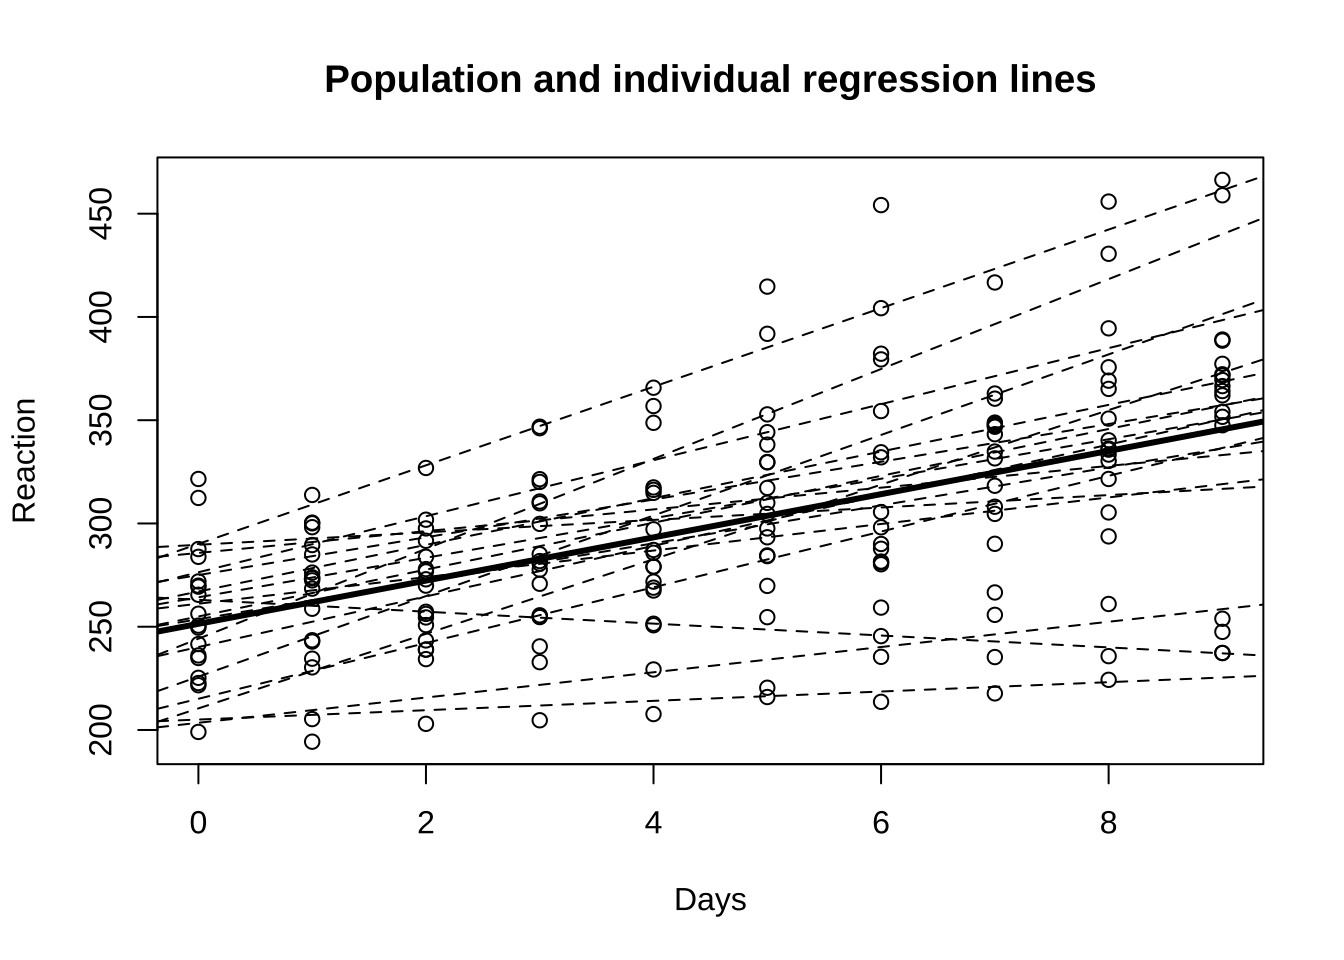
\includegraphics{repeat_files/figure-latex/pmodel-1.pdf}

이제 각 운전사에 대하여 개체별로 적합한 회귀식의 계수들\((\hat \beta_{0i}, \hat \beta_{1i})\) 와 전체집단에 적한한 회귀식의 계수 \((\hat \beta_{0}, \hat \beta_{1})\)의 관계를 보면 개체별로 회귀 계수들의 평균이 전체에 적용한 모형의 계수와 매우 가까운 사실을 알 수 있다.

\begin{Shaded}
\begin{Highlighting}[]
\FunctionTok{apply}\NormalTok{(}\FunctionTok{coef}\NormalTok{(lmf1),}\DecValTok{2}\NormalTok{,mean)}
\end{Highlighting}
\end{Shaded}

\begin{verbatim}
## (Intercept)        Days 
##   251.40510    10.46729
\end{verbatim}

\begin{Shaded}
\begin{Highlighting}[]
\FunctionTok{coef}\NormalTok{(lmpop)}
\end{Highlighting}
\end{Shaded}

\begin{verbatim}
## (Intercept)        Days 
##   251.40510    10.46729
\end{verbatim}

\hypertarget{uxc784uxc758-uxacc4uxc218-uxbaa8uxd615}{%
\subsection{임의 계수 모형}\label{uxc784uxc758-uxacc4uxc218-uxbaa8uxd615}}

앞 절의 모형과 분석에서 알 수 있듯이 한 개체에 대하여 여러 개의 관측값을 측정한 자료에 회귀방정식을 각각 적합시켜보고 또한 개체의 특성을 고려하지않은 전체 모형을 적합해보면 다음과 같은 두 가지 결과를 볼 수 있다.

\begin{itemize}
\tightlist
\item
  각 개체별 회귀식은 개인의 특성을 반영한다. 즉, 개체에 따라 시간에 따른 반응시간의 변화가 다르게 나타난다.
\item
  하지만 개인별로 볼 때도 전체적으로는 시간에 따라서 반응시간이 증가하는 경향이 있음을 알 수 있다.
\item
  전체 자료에 적합한 모형을 보면 개인별로 적합한 모형의 공통적인 성격, 즉 시간에 따른 반응시간의 증가를 알 수 있다.
\item
  이러한 결과를 보고 각 개인의 변화는 전체적인 변화를 따르면서 각 개인의 특성이 반영되었다고 가정할 수 있다.
\end{itemize}

위에서 논의하였듯이 전체적인 경향과 게인의 특성을 동시에 고려할 수 있는 모형이 생각할 수 있고 이러한 모형이 다음과 같은 모형이다.

\begin{equation} 
y_{ij} = (\beta_0 + b_{0i}) + (\beta_1 + b_{1i}) t_j + e_{ij} 
\label{eq:repeat}
\end{equation}

모형 \$ref(eq:repeat) 는 절편과 기울기가 두 개의 구성 요소로 더해져서 표현된다.기울기는 \(\beta_1+b_{1i}\)로서 나타내어지며 \(\beta_1\)은 모집단이 가지는 공통적인 경향을 반영하는 모수이고 \(b_{1i}\)는 \(i\) 번째 개체의 특성을 반영한 확률변수이다. 절편도 유사한 형식으로 구성된다.
각 개인에 대한 특성을 나타내는 변수 \((b_{0i}, b_{1i})\) 을 확률변수로 설정하고 이를 모수(\(\beta_0, \beta_1)\) (parameter or fixed effect)와 구별하여 임의효과(random effect)라고 한다.

위와 같이 선형모형의 계수에 각 개체에 대한 임의효과가 포함된 모형을 특별하게
\textbf{임의 계수 모형(random coefficient model)} 이라고 부른다.

18명에 대한 회귀직선의 절편과 기울기를 보면 개인의 차이에 따른 변동을 볼 수 있으며 이러한 각 개인간의 변동을 임의효과 를 이용하여 다음과 같은 모형을 생각해보자.

\[
\bm \beta_i=
\left[ \begin{array}{c}
\beta_{0} \\
\beta_{1} \\
\end{array} \right]
+\left[ \begin{array}{c}
b_{0i} \\
b_{1i} \\
\end{array} \right]
, \quad
\left[ \begin{array}{c}
b_{0i} \\
b_{1i} \\
\end{array} \right] \sim
N \left (
\left[ \begin{array}{c}
0 \\
0 \\
\end{array} \right]
,
\left[ \begin{array}{cc}
\sigma^2_{b1} & \rho \sigma_{b1} \sigma_{b2}\\
\rho \sigma_{b1} \sigma_{b2} & \sigma^2_{b2} \\
\end{array} \right]
\right )
\]

위의 모형은 각 개인의 회귀직선에서 각 절편과 기울기가 전체평균 \(\beta_0\)와 \(\beta_1\)를 따르며 각 개인의 차이는 전체평균에 임의효과인 \(b_{0i}\)와 \(b_{1i}\)가 더해져서 나타난다는 것을 의미한다. 이변량 임의효과 \(b_{0i}\)와 \(b_{1i}\)는 이변량 정규분포를 따르며 각각의 분산과 상관계수가 \(\sigma^2_{b1}\), \(\sigma^2_{b2}\), \(\rho\)이다.

다른 개체에 대한 임의효과는 서로 독립이며 임의 효과와 오차항은 독립이다. 여기서 오차항은 서로 독립이며 \(N(0, \sigma^2_e)\)를 따른다고 가정한다.

\[ Cov(\bm b_{i}, \bm b_{j}) =\bm 0 \text{ when } i \ne j,\quad
Cov(\bm b_{i}, e_{jk}) =\bm 0 \text{ for all } i,j,k \]

위와 같은 혼합효과모형(mixed effects model)을 각 개인 \(i\)에 대하여 행렬식으로 표시하면 다음과 같다.

\begin{equation}
\bm y_i = \bm X_i \bm \beta + \bm Z_i \bm b_i + \bm e_i 
\label{eq:indilm}
\end{equation}

여기서

\[ 
\bm y_i=\left[ \begin{array}{c}
y_{i1} \\
y_{i2} \\
\vdots \\
y_{i,10}
\end{array} \right],~\bm X_i =
\left[ \begin{array}{cc}
1 & 0 \\
1 & 1 \\
\vdots & \vdots  \\
1 & 9 
\end{array} \right], \bm  \beta=
\left[ \begin{array}{c}
\beta_{0} \\
\beta_{1} \\
\end{array} \right], ~\bm Z_i =
\left[ \begin{array}{cc}
1 & 0 \\
1 & 1 \\
\vdots & \vdots  \\
1 & 9 
\end{array} \right],~ \bm b_i =
\left[ \begin{array}{c}
b_{0i} \\
b_{1i} \\
\end{array} \right],~
\bm  e_i= 
\left[ \begin{array}{c}
e_{i1} \\
e_{i2} \\
\vdots \\
e_{i,10}
\end{array} \right]
\]

그리고 각 개인에 대한 임의 효과 \(\bm b_i\)와 오차항 벡터 \(\bm e_i\)의 공분산행렬은 다음과 같다

\[
Cov(\bm b_i) = \bm \Sigma =
\begin{bmatrix}
\sigma^2_{b1} & \rho \sigma_{b1} \sigma_{b2}\\
\rho \sigma_{b1} \sigma_{b2} & \sigma^2_{b2} 
\end{bmatrix}, \quad
Cov(\bm e_i) = \sigma-e^2
 \bm I
\]

위의 각 개인에 대한 모형 \eqref{eq:indilm} 을 모두 합쳐서 하나의 혼합효과모형 으로 나타내면 식 \eqref{eq:mixedmodel} 과 같이 다음과 같이 표현할 수 있다.

\begin{equation*}
\bm  y = \bm  X \bm \beta + \bm Z \bm b + \bm e 
\end{equation*}

여기서

\[ 
\bm y=\left[ \begin{array}{c}
\bm y_{1} \\
\bm y_{2} \\
\vdots \\
\bm y_{18}
\end{array} \right],~\bm X =
\left[ \begin{array}{c}
\bm X_1 \\
\bm X_2 \\
\vdots   \\
\bm  X_{18} 
\end{array} \right]
~ \bm e =
\left[ \begin{array}{c}
\bm e_1 \\
\bm e_2 \\
\vdots  \\
\bm e_{18} 
\end{array} \right]
\]

임의효과 벡터 \(\bm b\)는 각 개인에 대한 임의효과벡터 \(\bm b_i\)를 행으로 쌓아놓은것과 같고 임의효과에 대한 계획행렬 \(\bm Z\)는 각 개인의 계획행렬 \(\bm Z_i\)를 대각원소로 같은 행렬이다.

\[
\bm b=\left[ \begin{array}{c}
\bm b_{1} \\
\bm b_{2} \\
\vdots \\
\bm b_{18}
\end{array} \right],~\bm Z =
\left[ \begin{array}{cccc}
\bm Z_1 & 0 & \dots & 0 \\
0   & \bm Z_2 & \dots & 0 \\
\vdots & \vdots & \vdots & \vdots  \\
0 & 0 & \dots & \bm Z_{18}
\end{array} \right]
\]

또한 임의효과 벡터 \(\bm b\) 와 오차항 벡터 \(\bm e\)의 공분산행렬은 다음과 같다.

\[ 
Cov(\bm b) = \bm G = 
\begin{bmatrix}
\bm \Sigma & 0 & \dots & 0 \\
0   & \bm \Sigma & \dots & 0 \\
\vdots & \vdots & \vdots & \vdots  \\
0 & 0 & \dots & \bm \Sigma
\end{bmatrix}, \quad
Cov(\bm e) = \bm R = \sigma_e^2 \bm I
\]

혼합모형 @ref\{eq:mixed)를 \texttt{lmer()} 함수를 이용하여 적합시켜보자. 모형에서 \texttt{(1\ +\ Days\textbar{}Subject)} 이 개체에 대하여 절편과 기울기에 대한 임의효과를 지정한다.

\begin{Shaded}
\begin{Highlighting}[]
\NormalTok{fm1 }\OtherTok{\textless{}{-}} \FunctionTok{lmer}\NormalTok{(Reaction }\SpecialCharTok{\textasciitilde{}} \DecValTok{1} \SpecialCharTok{+}\NormalTok{ Days }\SpecialCharTok{+}\NormalTok{ (}\DecValTok{1} \SpecialCharTok{+}\NormalTok{ Days}\SpecialCharTok{|}\NormalTok{Subject), sleepstudy)}
\FunctionTok{summary}\NormalTok{(fm1)}
\end{Highlighting}
\end{Shaded}

\begin{verbatim}
## Linear mixed model fit by REML ['lmerMod']
## Formula: Reaction ~ 1 + Days + (1 + Days | Subject)
##    Data: sleepstudy
## 
## REML criterion at convergence: 1743.6
## 
## Scaled residuals: 
##     Min      1Q  Median      3Q     Max 
## -3.9536 -0.4634  0.0231  0.4634  5.1793 
## 
## Random effects:
##  Groups   Name        Variance Std.Dev. Corr
##  Subject  (Intercept) 612.10   24.741       
##           Days         35.07    5.922   0.07
##  Residual             654.94   25.592       
## Number of obs: 180, groups:  Subject, 18
## 
## Fixed effects:
##             Estimate Std. Error t value
## (Intercept)  251.405      6.825  36.838
## Days          10.467      1.546   6.771
## 
## Correlation of Fixed Effects:
##      (Intr)
## Days -0.138
\end{verbatim}

\hypertarget{sasuxc758-proc-mixed}{%
\section{\texorpdfstring{\texttt{SAS}의 \texttt{proc\ mixed}}{SAS의 proc mixed}}\label{sasuxc758-proc-mixed}}

\texttt{SAS}에서 혼합모형을 적함시키는 방법은 여러 가지 있지만 대표적인 방법이
\texttt{proc\ mixed}를 사용하는 것이다.

다시 앞에서 본 반복큭정에 대한 모형식 \eqref{eq:repeatmodel0}를 고려하자.

\[
y_{ijk} = \mu + \alpha_i + \beta_{ij} + \gamma_k + \delta_{ik} + e_{ijk} 
\]

위의 모형은 \texttt{proc\ mixed}를 이용하여 다음과 같이 적합시킬 수 있다.

\begin{verbatim}
proc mixed data=bp;
   class trt time id;
   model bp = trt time trt*time;
   repeated / type=cs sub=id;
run;
\end{verbatim}

위의 \texttt{proc\ mixed} 프로그램은 \texttt{proc\ glm}의 문법과 매우 동일하지만 \texttt{repeated} 문장에서 효과를 주지 않고 option으로 오차항의 공분산 행렬 \(R\) 의 형태를 지정하는 \texttt{type=cs} 사용한다. 또한 반복측정하는 개체(subject)의 단위를 \texttt{sub=id} 로 지정한다.

\texttt{proc\ mixed} 의 \texttt{repeated} 를 사용하면 개체 내의 자료에 대한 다양한 형태의 공분산 \(\bm R\) 을 지정할 수 있다. 다양한 공분산의 형태는 \href{https://documentation.sas.com/doc/en/pgmsascdc/9.4_3.3/statug/statug_mixed_syntax14.htm}{SAS 매뉴얼} 에 나와 있다.

위에서 지정한 오차항의 공분산 행렬 \(R\) 의 형태는 compound symmetry(cs)이며 이는 개체 내의 반복측정한 반응값이 같은 공분산을 가지는 형태이다. 이러한 모형은 \texttt{proc\ mixed} 에서 다음과 같이 \texttt{random} 문장을 사용하여 동일하게 지정할 수 있다.

\begin{verbatim}
proc mixed data=bp ;
   class trt time id;
   model bp=trt time trt*time / ddfm=kr;
   random  int / sub=id;
run;
\end{verbatim}

위에서 \texttt{random} 문장은 혼함모형 식 \eqref{eq:mixedmodel}에서 절편(intercent)에 각 개체의 임의효과를 더한 모형이며 이는 반복 츧정에 대한 선형모형식
@ref\{eq:repeatmodel0\}에서 개체의 효과 \(\beta_{ij}\)를 임의효과로 보는 모형이다. 앞에서 논의한 임의게수 모형에서 절편에만 임의효과가 있는 모형과 유사하다.

이렇게 모형식 @ref\{eq:repeatmodel0\}에서 절편에만 임의효과가 있고 오차항이 독립인 모형은 모형식 @ref\{eq:repeatmodel0\}에서 모든 모수를 고정효과로 보고 개체안의 오차항에 대한 공분산이 compound symmetry 라고 가정하는 모형과 주변 분포가 동일하다.

따라서 위의 두 개 의 \texttt{SAS}의 가설 검정 결과는 같다. 더 나아가 \texttt{proc\ glm}을 이용항 결과와도 동일하다.

\hypertarget{crossover1}{%
\chapter{교차실험 1}\label{crossover1}}

보통 의학실험은 2개 이상의 처리를 각각 독립적인 집단에 적용하는 병렬계획(parallel design)을 사용한다. 즉 환자는 랜덤화 이후 지정된 한 개의 처리만을 받는다. 이러한 병렬계획과는 다르게 한 명의 환자가 2개 이상의 처리를 받는 실험이 있는데 이를 \textbf{교차계획(crossover design)} 이라고 부른다.

\hypertarget{uxad50uxacfc-uxc608uxc81c-6.2}{%
\section{교과 예제 6.2}\label{uxad50uxacfc-uxc608uxc81c-6.2}}

교과서 예제 6.2 에 논의된 자료는 지금까지논의한 실험과 매우 다른 교차계획을 사용하였다.
고려된 요인은 약의 농도이며 처리는 3개다(2mg, 3mg, 4mg). 또한 각 처리에 대하여 심전도를 8번을 반복측정 하였다.
주목할 점은 1명의 환자가 3개의 처리를 순차적(1주일 간격)으로 모두 받았다는 점이다. 따라서 이는 교차계획을 이용한 실험이다.

이 실험에서 주요 분석 사항은 다음과 같다.

\begin{itemize}
\tightlist
\item
  성별에 대한 차이?
\item
  농도와 시간에 따라서 심전도가 차이가 있는가?
\item
  농도와 시간간의 차이가 있는가?
\end{itemize}

이 실험에 대한 모형은 다음과 같다.

\hypertarget{uxbaa8uxd615-1}{%
\subsection{모형}\label{uxbaa8uxd615-1}}

\begin{equation}
y_{ijkl} = ( \mu + b_{0l} ) + \alpha_i + ( \beta_j + b_{1jl} ) + (\gamma_k  + b_{2kl})  + (\alpha \beta)_{ij} + 
(\alpha \gamma)_{ik} + (\beta \gamma)_{jk} + (\alpha \beta \gamma)_{ijk}  + e_{ijkl}
\label{eq:ex62model}
\end{equation}

위의 모형에서 고정효과는 다음과 같다.

\begin{longtable}[]{@{}lll@{}}
\toprule
고정효과 & 의미 & 비고\tabularnewline
\midrule
\endhead
\(\alpha_i\) & 성별 효과 & \(i=1,2\)\tabularnewline
\(\beta_j\) & 약의 농도 효과 & \(j=1,2,3\)\tabularnewline
\(\gamma_k\) & 시간 효과 & \(k=1,2,..,8\)\tabularnewline
\((\alpha \beta)_{ij}\) & 성별과 약농도 교효작용 효과 &\tabularnewline
\((\alpha \gamma)_{ik}\) & 성별과 시간 교효작용 효과 &\tabularnewline
\((\beta \gamma)_{jk}\) & 약농도와 시간 교효작용 효과 &\tabularnewline
\((\alpha \beta \gamma)_{ijk}\) & 성별/약농도/시간 교효작용 효과 &\tabularnewline
\bottomrule
\end{longtable}

또한 임의 효과는 다음과 같이 나타난다.

\begin{longtable}[]{@{}lll@{}}
\toprule
임의 효과 & 의미 & 비고\tabularnewline
\midrule
\endhead
\(b_{0l}\) & \(l\) 번째 환자에 대한 효과 & \(l=1,2,..12\)\tabularnewline
\(b_{1jl}\) & \(l\) 번째 환자의 농도에 대한 효과 & \(j=1,2,3, l=1,2,..12\)\tabularnewline
\(b_{2kl}\) & \(l\) 번째 환자의 시간에 대한 효과 & \(k=1,2,..8,l=1,2,..12\)\tabularnewline
\bottomrule
\end{longtable}

임의효과와 오차항의 분포는 다음과 같으며 모두 독립니다.

\begin{equation}
b_{0l} \sim N(0, \sigma_1^2), \quad 
b_{1jl} \sim N(0, \sigma_2^2), \quad
b_{2kl} \sim N(0, \sigma_3^2), \quad
e_{ijkl} \sim N(0, \sigma_e^3)
\label{eq:ex62random}
\end{equation}

\hypertarget{sas}{%
\subsection{SAS}\label{sas}}

예제 6.2의 모형식 \eqref{eq:ex62model} 을 \texttt{SAS} 의 \texttt{proc\ mixed} 로 적합하는 프로그램은 다음과 같다.

\begin{verbatim}
proc mixed data=hp01;
class gender hour  trt id;
model response=gender hour trt gender*hour gender*trt  hour*trt  gender*trt*hour/ ddfm=kr;
random  int trt hour/ subject=id;
run;
\end{verbatim}

예제 6.2의 모형식 \eqref{eq:ex62model} 을 \texttt{SAS} 의 \texttt{proc\ glm} 로 적합하는 프로그램은 다음과 같다.
아래 SAS 프로그램은 넓은 형식의 자료에 대한 프로그램이다.

\begin{verbatim}
PROC GLM data=hp0;
  CLASS Gender;
  MODEL Trt1_Hr_1--Trt3_Hr_8 =Gender/NOUNI SS3;
  REPEATED Trt 3(1 2 3), Hr 8(1 2 3 4 5 6 7 8 ) /PRINTE;
 RUN;
\end{verbatim}

\hypertarget{crossover2}{%
\chapter{교차실험 2}\label{crossover2}}

\hypertarget{uxac1cuxc694-1}{%
\section{개요}\label{uxac1cuxc694-1}}

앞장에서 한 명의 환자가 2개 이상의 처리를 받는 실험이 있는데 이를 \textbf{교차계획(crossover design)} 이라고 하였다.

교차계획으로 실험을 하는 경우 앞의 처리 효과가 두의 처리 효과에 영향을 미칠 수 있다.
따라서 하나의 처리응 적용한 후에 그 효과가 없어질 때까지 기다리는 기간이 필요하다.
이러한 기간을 휴약기간(washout period)이라고 한다.

이렇게 휴역기간이 있더라도 앞의 처리가 뒤의 처리에 영향을 미칠 수 있기 떄문에
교차계획에서는 환자를 랜덤하게 \textbf{처리 순서(sequence)} 중 하나에 배정한다.

예를 들어 두개의 약 A, B 을 처리로 하는 교차계획을 고려하자.
두 개의 처리 순서는 다음과 같다.

\begin{itemize}
\tightlist
\item
  순서 1: A 약을 복용하고 휴약시간을 가진 뒤에 B약을 복용
\item
  순서 2: B 약을 복용하고 휴약시간을 가진 뒤에 A약을 복용
\end{itemize}

한자는 위의 두 개의 순서 중 하나를 랜덤하게 배정받아서 실험에 참가하게 된다.
이러한 처리 순서를 랜덤하게 하는 이유는 처리의 배정 순서에 따른 효과가 있는 경우 이를
모형에 넣어서 처리 효과와 분리하려눈 것이다.

또한 처리를 받는 \textbf{시점(period)}도 고려해야할 효과이다. 어떤 처리든 먼저 받는 것과 나중에 받는 것의 효과가 다를 수 있다.

처리순서가 있는 교차실험 중에 2개의 순서(sequence)와 2개의 시점(period)가 있는 가장 단순한 실험 계획(\(2 \times 2\) 교차실험이라고 한다)을 도식화 하면 아래 그림과 같다.

\begin{figure}
\centering
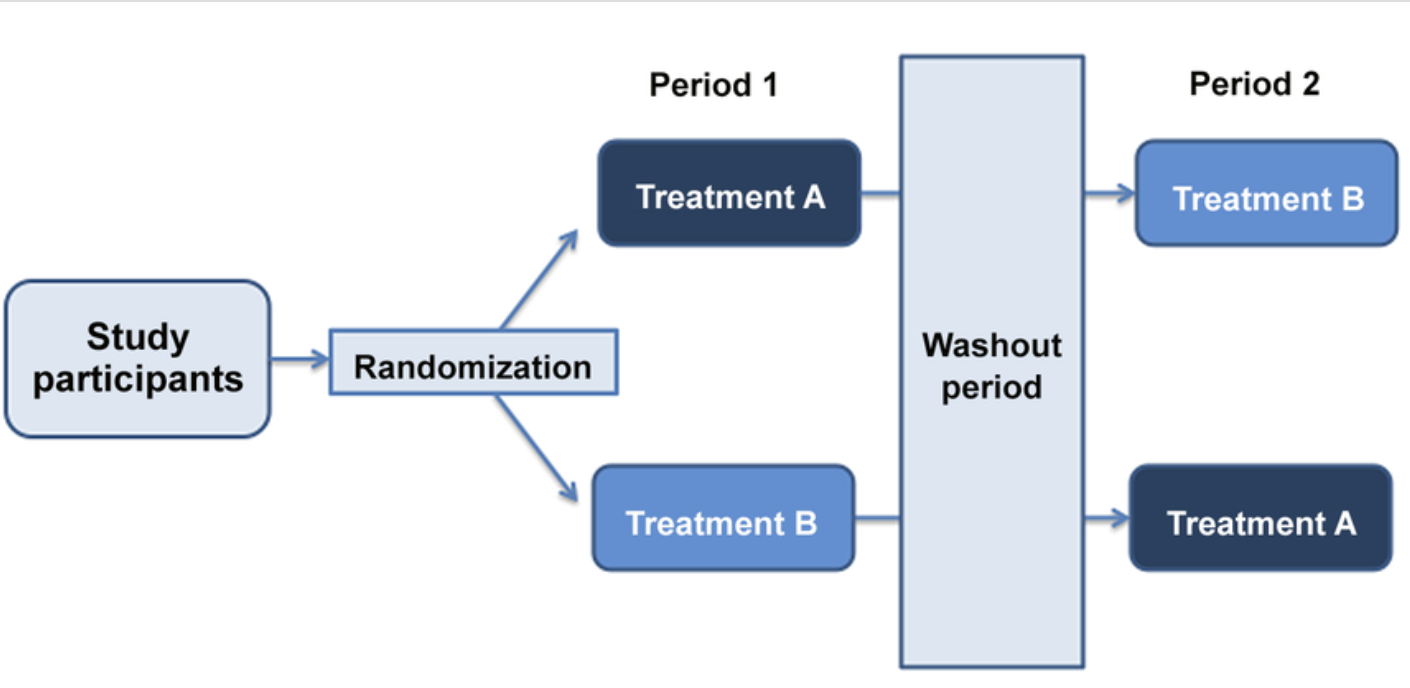
\includegraphics{cross1.png}
\caption{\(2 \times 2\) 교차실험}
\end{figure}

만약 시점을 4개 늘려서 처리를 2번 씩 반복한다면 \(2 \times 4\) 교차실험이이 된다. 이렇게 순서의 개수가 \(s\)과 시점의 수가 \(p\) 인 교차실험은 \(s \times p\) 교차살험이라고 부른다.

\begin{figure}
\centering
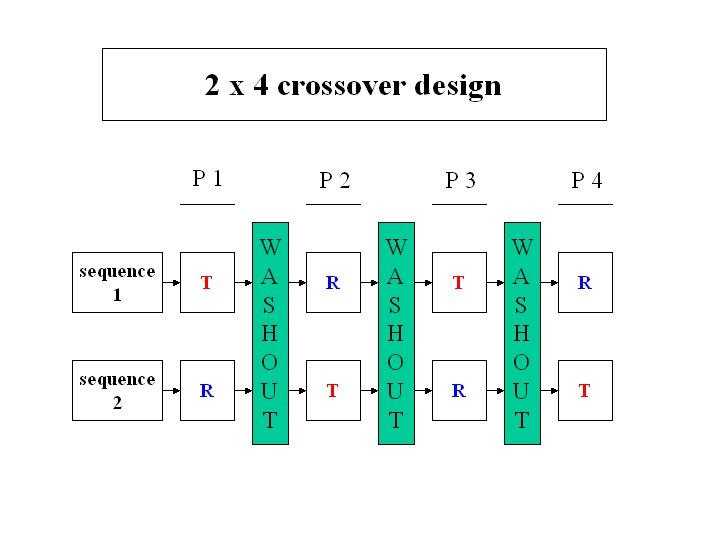
\includegraphics{design24.jpg}
\caption{\(2 \times 4\) 교차실험}
\end{figure}

\hypertarget{uxad50uxcc28uxc2e4uxd5d8uxc758-uxc7a5uxb2e8uxc810}{%
\section{교차실험의 장단점}\label{uxad50uxcc28uxc2e4uxd5d8uxc758-uxc7a5uxb2e8uxc810}}

교차실험은 다음과 같은 장점이 있다.

\begin{itemize}
\tightlist
\item
  병행계획(parallel design)보다 실험자의 수가 작다.
\end{itemize}

하지만 교차실험은 다음과 같은 단점들 때문에 쉽게 사용할 수 있다.

\begin{itemize}
\tightlist
\item
  치료가 되는 질환이 아닌 만성질환에만 적용이 가능하다.
\item
  앞의 치료기 뒤의 치료에 양향을 줄 수 있다 (\textbf{carry-over effect})
\item
  실험의 관리가 어렵다.
\end{itemize}

\hypertarget{uxad50uxcc28uxc2e4uxd5d8-uxbaa8uxd615}{%
\section{교차실험 모형}\label{uxad50uxcc28uxc2e4uxd5d8-uxbaa8uxd615}}

\(s \times p\) 교차실험에서 얻은 반응값 \(y_{ijk}\)에 대하여 일반적으로 다음과 같은 모형으로 기술된다.
아래 모형은 상호작용과 carry-over 효과를 고려하지 않은 가장 단순한 모형이다.

\begin{equation}
y_{ijkl} = \mu + \pi_j + \tau_{d(i,j)}  + s_{ik}  + e_{ijk} 
\label{eq:crossmodel2}
\end{equation}

\begin{longtable}[]{@{}lll@{}}
\toprule
요소 & 의미 & 비고\tabularnewline
\midrule
\endhead
\(\mu\) & 총평균(절편) &\tabularnewline
\(\pi_j\) & 시점 \(j\)에 대한 효과 & \(j=1,2,\dots,p\)\tabularnewline
\(\tau_{d(i,j)}\) & 순서 \(i\)의 시점 \(j\) 에 배정된 처리 효과 & \(i=1,2,\dots,s, j=1,2,\dots,p\)\tabularnewline
\(s_{ik}\) & 순서 \(i\)안에 있는 \(k\) 번쨰 개체의 효과 & \(i=1,2,\dots,s, k=1,2,\dots, n_i\)\tabularnewline
\(e_{ijk}\) & 오차항 &\tabularnewline
\bottomrule
\end{longtable}

순서 \(i\)안에 있는 \(k\) 번쨰 개체의 효과 \(s_{ik}\) 는 보통 임의효과로 놓은다. 임의효과와 오차항의 분포는 다음과 같다.

\[ s_{ik} \sim N(0, \sigma_s^2), \quad e_{ijk} \sim N(0, \sigma_e^2) \]

에를 들어서 위의 그림 \(2 \times 2\) 교차실험에서와 같이 순서 1 에서 (A,B) 로 처리를 주고(\(n_1\)명이 배정) 순서 2에서 (B,A)로 처리를 주면(\(n_2\)명이 배정) 반응값은 다음과 같이 나타낼 수 있다.

\begin{align*}
y_{11k} & = \mu + \pi_1 + \tau_A + s_{1k} + e_{11k}, \quad k=1,2,\dots, n_1 \\
y_{12k} & = \mu + \pi_2 + \tau_B + s_{1k} + e_{12k}, \quad k=1,2,\dots, n_1 \\
y_{21k} & = \mu + \pi_1 + \tau_B + s_{2k} + e_{21k}, \quad k=1,2,\dots, n_2 \\
y_{22k} & = \mu + \pi_2 + \tau_A + s_{2k} + e_{22k}, \quad k=1,2,\dots, n_2 
\end{align*}

이러한 교차실험에서는 다음과 같은 가설검정이 중요하다.

\begin{itemize}
\tightlist
\item
  처리간의 차이가 있는가?
\item
  시점의 차이가 있는가?
\end{itemize}

\hypertarget{sas-uxc758-proc-mixed}{%
\section{\texorpdfstring{\texttt{SAS} 의 \texttt{proc\ mixed}}{SAS 의 proc mixed}}\label{sas-uxc758-proc-mixed}}

위의 모형 \eqref{eq:crossmodel2}에 대한 \texttt{SAS} 의 \texttt{proc\ mixed} 프로그램은 다음과 같다.

\begin{verbatim}
PROC MIXED data=asthma;
  CLASS SEQUENCE SUBJECT PERIOD DRUG;
  MODEL PEF = DRUG  PERIOD;
  RANDOM SUBJECT;
  LSMEANS DRUG / PDIFF CL E;
run;
\end{verbatim}

  \bibliography{book.bib,packages.bib}

\end{document}
